% Options for packages loaded elsewhere
\PassOptionsToPackage{unicode}{hyperref}
\PassOptionsToPackage{hyphens}{url}
\PassOptionsToPackage{dvipsnames,svgnames,x11names}{xcolor}
%
\documentclass[
  sn-mathphys-num,
]{sn-jnl}



\usepackage{amsmath,amssymb}
\usepackage{iftex}
\ifPDFTeX
  \usepackage[T1]{fontenc}
  \usepackage[utf8]{inputenc}
  \usepackage{textcomp} % provide euro and other symbols
\else % if luatex or xetex
  \usepackage{unicode-math}
  \defaultfontfeatures{Scale=MatchLowercase}
  \defaultfontfeatures[\rmfamily]{Ligatures=TeX,Scale=1}
\fi
\usepackage{lmodern}
\ifPDFTeX\else  
    % xetex/luatex font selection
\fi
% Use upquote if available, for straight quotes in verbatim environments
\IfFileExists{upquote.sty}{\usepackage{upquote}}{}
\IfFileExists{microtype.sty}{% use microtype if available
  \usepackage[]{microtype}
  \UseMicrotypeSet[protrusion]{basicmath} % disable protrusion for tt fonts
}{}
\makeatletter
\@ifundefined{KOMAClassName}{% if non-KOMA class
  \IfFileExists{parskip.sty}{%
    \usepackage{parskip}
  }{% else
    \setlength{\parindent}{0pt}
    \setlength{\parskip}{6pt plus 2pt minus 1pt}}
}{% if KOMA class
  \KOMAoptions{parskip=half}}
\makeatother
\usepackage{xcolor}
\setlength{\emergencystretch}{3em} % prevent overfull lines
\setcounter{secnumdepth}{-\maxdimen} % remove section numbering
% Make \paragraph and \subparagraph free-standing
\makeatletter
\ifx\paragraph\undefined\else
  \let\oldparagraph\paragraph
  \renewcommand{\paragraph}{
    \@ifstar
      \xxxParagraphStar
      \xxxParagraphNoStar
  }
  \newcommand{\xxxParagraphStar}[1]{\oldparagraph*{#1}\mbox{}}
  \newcommand{\xxxParagraphNoStar}[1]{\oldparagraph{#1}\mbox{}}
\fi
\ifx\subparagraph\undefined\else
  \let\oldsubparagraph\subparagraph
  \renewcommand{\subparagraph}{
    \@ifstar
      \xxxSubParagraphStar
      \xxxSubParagraphNoStar
  }
  \newcommand{\xxxSubParagraphStar}[1]{\oldsubparagraph*{#1}\mbox{}}
  \newcommand{\xxxSubParagraphNoStar}[1]{\oldsubparagraph{#1}\mbox{}}
\fi
\makeatother


\providecommand{\tightlist}{%
  \setlength{\itemsep}{0pt}\setlength{\parskip}{0pt}}\usepackage{longtable,booktabs,array}
\usepackage{calc} % for calculating minipage widths
% Correct order of tables after \paragraph or \subparagraph
\usepackage{etoolbox}
\makeatletter
\patchcmd\longtable{\par}{\if@noskipsec\mbox{}\fi\par}{}{}
\makeatother
% Allow footnotes in longtable head/foot
\IfFileExists{footnotehyper.sty}{\usepackage{footnotehyper}}{\usepackage{footnote}}
\makesavenoteenv{longtable}
\usepackage{graphicx}
\makeatletter
\def\maxwidth{\ifdim\Gin@nat@width>\linewidth\linewidth\else\Gin@nat@width\fi}
\def\maxheight{\ifdim\Gin@nat@height>\textheight\textheight\else\Gin@nat@height\fi}
\makeatother
% Scale images if necessary, so that they will not overflow the page
% margins by default, and it is still possible to overwrite the defaults
% using explicit options in \includegraphics[width, height, ...]{}
\setkeys{Gin}{width=\maxwidth,height=\maxheight,keepaspectratio}
% Set default figure placement to htbp
\makeatletter
\def\fps@figure{htbp}
\makeatother

%%%% Standard Packages

\usepackage{graphicx}%
\usepackage{multirow}%
\usepackage{amsmath,amssymb,amsfonts}%
\usepackage{amsthm}%
\usepackage{mathrsfs}%
\usepackage[title]{appendix}%
\usepackage{xcolor}%
\usepackage{textcomp}%
\usepackage{manyfoot}%
\usepackage{booktabs}%
\usepackage{algorithm}%
\usepackage{algorithmicx}%
\usepackage{algpseudocode}%
\usepackage{listings}%

%%%%

\raggedbottom
\usepackage{multirow}
\usepackage{centernot}
\makeatletter
\@ifpackageloaded{caption}{}{\usepackage{caption}}
\AtBeginDocument{%
\ifdefined\contentsname
  \renewcommand*\contentsname{Table of contents}
\else
  \newcommand\contentsname{Table of contents}
\fi
\ifdefined\listfigurename
  \renewcommand*\listfigurename{List of Figures}
\else
  \newcommand\listfigurename{List of Figures}
\fi
\ifdefined\listtablename
  \renewcommand*\listtablename{List of Tables}
\else
  \newcommand\listtablename{List of Tables}
\fi
\ifdefined\figurename
  \renewcommand*\figurename{Figure}
\else
  \newcommand\figurename{Figure}
\fi
\ifdefined\tablename
  \renewcommand*\tablename{Table}
\else
  \newcommand\tablename{Table}
\fi
}
\@ifpackageloaded{float}{}{\usepackage{float}}
\floatstyle{ruled}
\@ifundefined{c@chapter}{\newfloat{codelisting}{h}{lop}}{\newfloat{codelisting}{h}{lop}[chapter]}
\floatname{codelisting}{Listing}
\newcommand*\listoflistings{\listof{codelisting}{List of Listings}}
\makeatother
\makeatletter
\makeatother
\makeatletter
\@ifpackageloaded{caption}{}{\usepackage{caption}}
\@ifpackageloaded{subcaption}{}{\usepackage{subcaption}}
\makeatother

\ifLuaTeX
  \usepackage{selnolig}  % disable illegal ligatures
\fi
\usepackage{bookmark}

\IfFileExists{xurl.sty}{\usepackage{xurl}}{} % add URL line breaks if available
\urlstyle{same} % disable monospaced font for URLs
\hypersetup{
  pdftitle={A mixture of hidden Markov models to predict the lymphatic spread in head and neck cancer depending on primary tumor location},
  colorlinks=true,
  linkcolor={blue},
  filecolor={Maroon},
  citecolor={Blue},
  urlcolor={Blue},
  pdfcreator={LaTeX via pandoc}}


\title[A mixture of hidden Markov models to predict the lymphatic spread
in head and neck cancer depending on primary tumor location]{A mixture
of hidden Markov models to predict the lymphatic spread in head and neck
cancer depending on primary tumor location}

% author setup
\author[1,2]{\fnm{Yoel Perez} \sur{Haas}}\email{yoel.perezhaas@usz.ch}\author*[1,2]{\fnm{Roman} \sur{Ludwig}}\email{roman.ludwig@usz.ch}\author[1,2]{\fnm{Julian} \sur{Brönnimann}}\author[1,2]{\fnm{Esmée Lauren} \sur{Looman}}\author[2]{\fnm{Panagiotis} \sur{Balermpas}}\author[11]{\fnm{Sergi} \sur{Benavente}}\author[3,4,7]{\fnm{Adrian} \sur{Schubert}}\author[8]{\fnm{Dorothea} \sur{Barbatei}}\author[8]{\fnm{Laurence} \sur{Bauwens}}\author[2]{\fnm{Jean-Marc} \sur{Hoffmann}}\author[3]{\fnm{Olgun} \sur{Elicin}}\author[6,10]{\fnm{Matthias} \sur{Dettmer}}\author[2]{\fnm{Bertrand} \sur{Pouymayou}}\author[4,5]{\fnm{Roland} \sur{Giger}}\author[8]{\fnm{Vincent} \sur{Grégoire}}\author[1,2]{\fnm{Jan} \sur{Unkelbach}}\email{jan.unkelbach@usz.ch}
% affil setup
\affil[1]{\orgdiv{Department of Physics}, \orgname{University of
Zurich}}
\affil[2]{\orgdiv{Radiation Oncology}, \orgname{University Hospital
Zurich}}
\affil[3]{\orgdiv{Department of Radiation Oncology}, \orgname{Bern
University Hospital}}
\affil[4]{\orgdiv{Department of ENT, Head \& Neck
Surgery}, \orgname{Bern University Hospital}}
\affil[5]{\orgdiv{Head and Neck Anticancer Center}, \orgname{Bern
University Hospital}}
\affil[6]{\orgdiv{Institute of Tissue Medicine and
Pathology}, \orgname{Bern University Hospital}}
\affil[7]{\orgdiv{Department of ENT, Head \& Neck
Surgery}, \orgname{Réseau Hospitalier Neuchâtelois}}
\affil[8]{\orgdiv{Department of Radiation Oncology}, \orgname{Centre
Léon Bérard}}
\affil[9]{\orgdiv{Department of Head and Neck Surgery}, \orgname{Centre
Léon Bérard}}
\affil[10]{\orgdiv{Institute of Pathology}, \orgname{Klinikum
Stuttgart}}
\affil[11]{\orgdiv{Departement of Radiation Oncology}, \orgname{Hospital
Vall d'Hebron}}

% abstract 

\abstract{Purpose: to be done

Methods: to be done

Results: to be done

Conclusions: to be done}

% keywords

\begin{document}
\maketitle


\section{Introduction}\label{introduction}

Head and Neck Squamous Cell Carcinoma (HNSCC) are known to spread
through the lymphatic system often leading to metastases in the lymph
nodes \citep[@shah\_patterns\_1990]{mukherji_cervical_2001}. To minimize
nodal recurrences, lymph node levels (LNL) at risk of harboring occult
metastases are typically irradiated electively. Current guidelines for
different tumor locations are based on the overall prevalence of nodal
disease as reported in literature
\citep[@mukherji\_cervical\_2001, @shah\_patterns\_1990]{biau_selection_2019}.

To personalize the prediction of the risk of occult metastases, given a
patient's individual diagnosis, we previously published a large,
multi-centric dataset where the lymphatic involvement per LNL is
available for each
patient\citep[@ludwig\_multi-centric\_2023]{ludwig_dataset_2022}.Building
on this dataset, we introduced an interpretable hidden Markov model
(HMM), trained to predict the risk for occult nodal disease, given an
individual patient's diagnosis \citep{ludwig_hidden_2021}.

Personalized risk predictions could enable clinicians to safely reduce
the elective clinical target volume (CTV-N), potentially decreasing
treatment-related side effects that impair a patient's quality of life,
without compromising the efficacy of the treatment
\citep{batth_practical_2014}.

Initially, separate models were trained for distinct tumor locations,
such as the oropharynx and oral cavity. These tumor locations are also
used in guidelines to define the elective target volumes
\citep{biau_selection_2019}. However, this approach did not account for
variations in lymphatic spread between subsites within these tumor
regions. With data for more than 2700 patients available, we can now
further analyze subsite specific spread patterns. Closer analysis showed
that pooling subsites into a single model led to inaccurate predictions,
as it failed to capture distinct lymphatic spread patterns. To resolve
this, we propose using a mixture of HMMs, which allows us to model the
lymphatic spread more accurately for tumors located near anatomical
borders, such as those between the oropharynx and oral cavity (e.g.,
tumors in the palate).

Additionally, we extend the analysis to a broader mixture model that
encompasses tumors of the oral cavity, oropharynx, hypopharynx, and
larynx, offering a more comprehensive understanding of lymphatic spread
across these regions.

\section{Data on Lymphatic Progression Patterns}\label{sec-data}

For the analyses in this work, we used seven datasets from 5
institutions resulting in 2741 patients in total.

\begin{enumerate}
\def\labelenumi{\arabic{enumi}.}
\tightlist
\item
  0 oropharyngeal patients from the University of Zurich in Switzerland
\item
  0 oropharyngeal patients from the Centre Léon Bérard in France
\item
  0 oropharyngeal, larynx and oral cavity patients from the Inselspital
  Bern in Switzerland
\item
  0 oropharyngeal, larynx and oral cavity patients from the Centre Léon
  Bérard in France
\item
  0 oropharyngeal, larynx and oral cavity patients from the University
  of Zurich in Switzerland
\item
  164 oropharyngeal patients from the Hospital Vall d'Hebron in Spain
  (not yet public)
\item
  979 hypopharynx, larynx and oral cavity patients from University
  Medical Center Groningen (not yet public)
\end{enumerate}

The datasets 1-4 are publicly available as CSV tables
(\citet{ludwig_multi-centric_2023} \citet{ludwig_detailed_2022}) and can
be interactively explored on \href{https://lyprox.org}{LyProX}. For each
patient the primary tumor subsite is reportd and each indicidual LNL is
reported as either metastatic or healthy given the available diagnostic
modalities, which include pathology after neck dissection in some
patients. In this work we will stratify the tumor locations into
different ICD codes which are depicted in figure~\ref{fig-subsites}.

\begin{figure}

\centering{

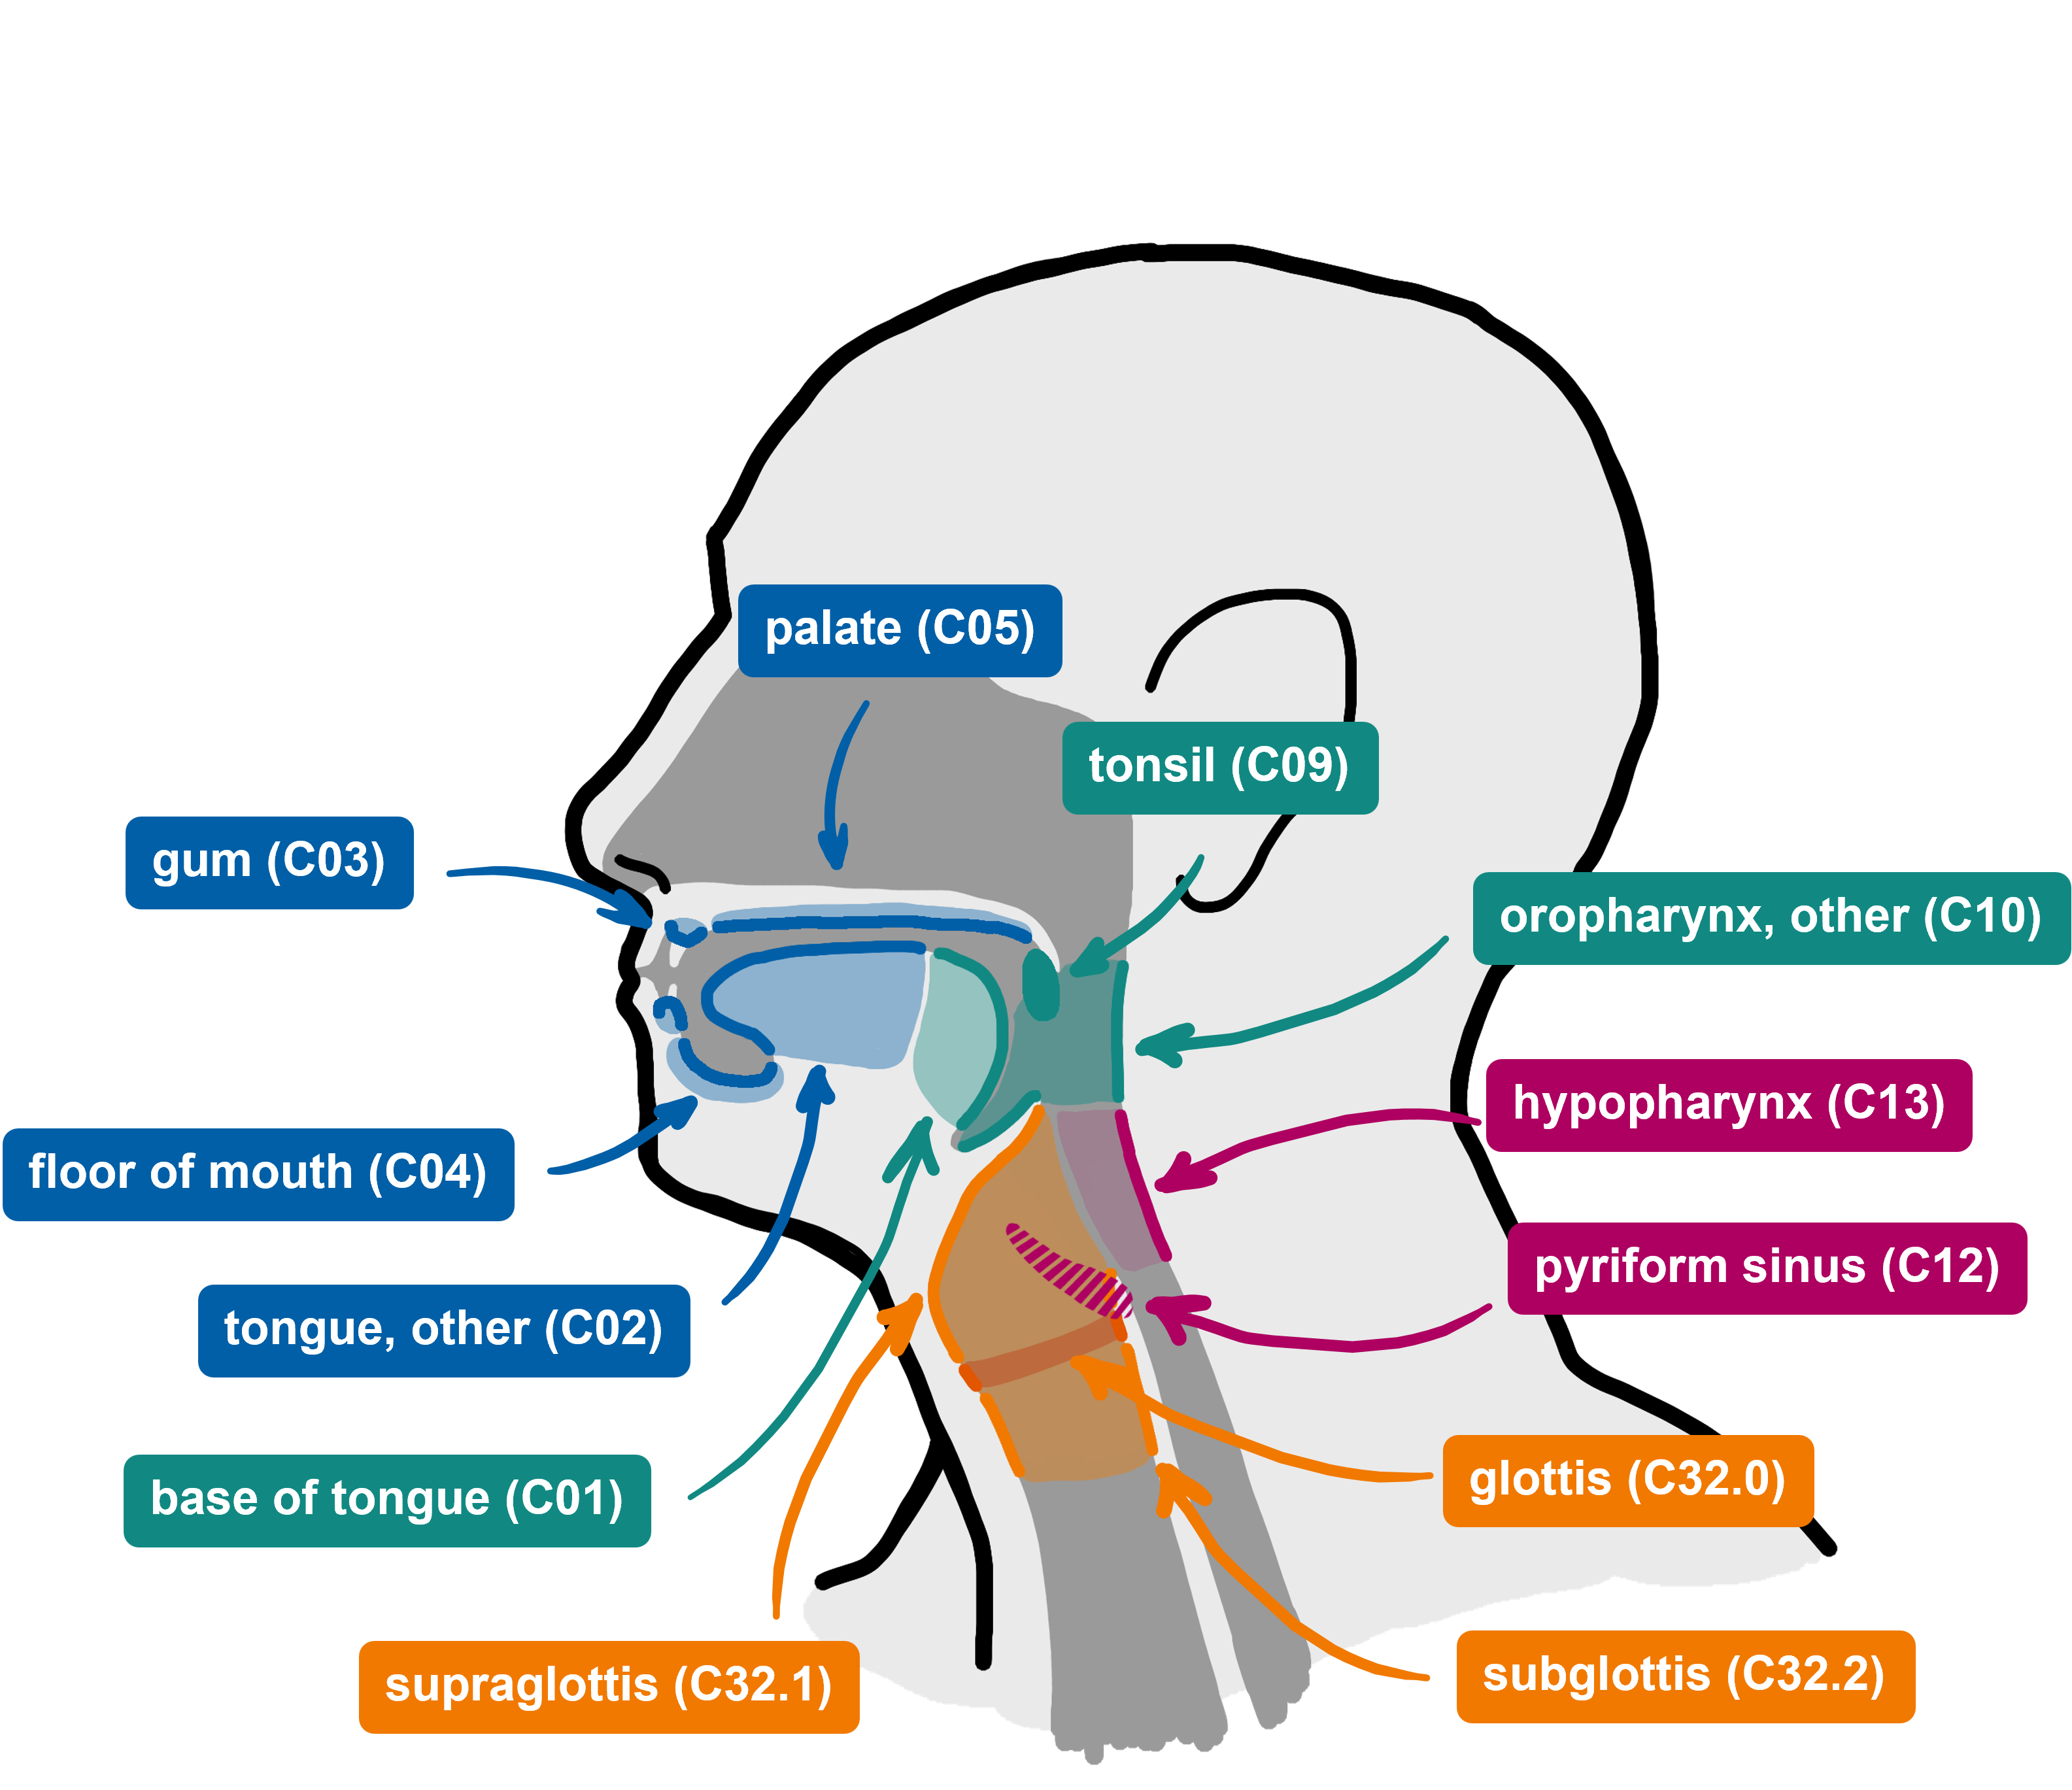
\includegraphics{figures/Subsites.png}

}

\caption{\label{fig-subsites}Anatomical sketch of the tumor subsites and
their corresponding ICD-10 codes. Subsite C06 ``other parts of mouth''
has not been included. Further the The tumor locations are color coded
in the following pattern: blue-oral cavity, green-oropharynx,
red-hypopharynx, orange-larynx.}

\end{figure}%

The prevelance of involvement in LNLs I, II, III, IV and V is shown in
figure~\ref{fig-involvement}. The involvement is stratified per tumor
subsite and t-stage. The figure illustrates the variations in LNL
involvement between subsites within oral cavity (blue), oropharynx
(green), hypopharynx (red) and larynx (orange). The involvement pattern
presents a continuous change over the tumor subsites. Where tumors in
the oral cavity show the most prominent LNL I involvement. As the tumor
location moves towards the oropharynx LNL II involvement increases.
Moving the tumor location further in caudal direction towards the
hypopharynx increases LNL III involvement while LNL I and II involvement
decrease. Larnygeal tumors show the least LNL I involvement.

\begin{figure}

\centering{

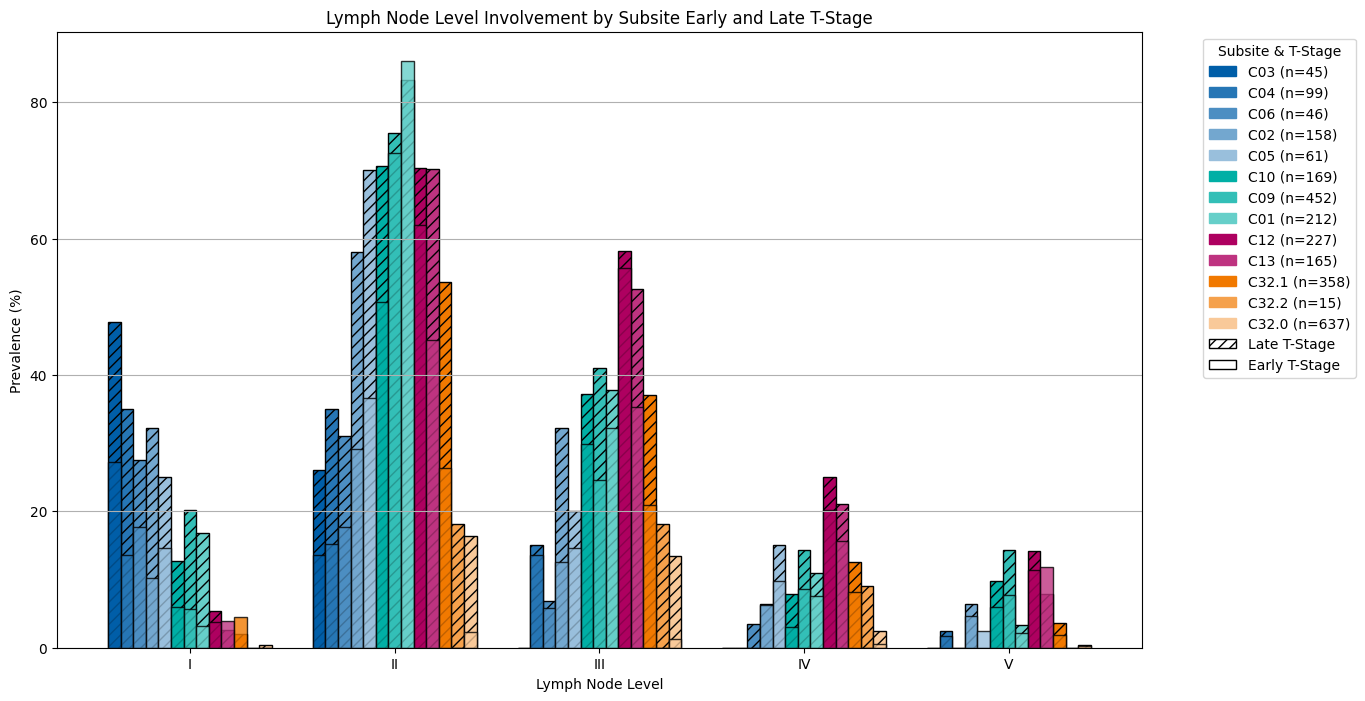
\includegraphics{figures/involvement_I_to_V_all_sites_t_staging.png}

}

\caption{\label{fig-involvement}Prevalence of ipsilateral LNL
involvement stratified by subsite. The subsites are sorted in natural
order to represent the continuously changing LNL involvement. The
different tumo locations are color coded, where oral cavity subsistes
are depicted in blue, larynx in green, hypopharynx in red and larynx in
orange. The patient data is further stratified in early t-stage (0-2)
and late t-stage (3-4). The legend furter specifies the number of
patients in each subsite.}

\end{figure}%

\section{Unilateral Model for Lymphatic
Progression}\label{sec-unilateral}

In this chapter we will briefly summarize unilateral model for
ipsilateral lymph node involvement introduced in
\citet{ludwig_hidden_2021}, presenting the notation which is then needed
to extend the HMM to a mixture model encompassing multiple tumor
subsites.

The HMM describes each LNL \(v \in 1, 2, ..., V\) by a binary random
variable corresponding to the status of the LNL; healthy (0) or involved
(1). The entire state of a patient with \(V\) LNLs is defined by the
\(v\)-dimensional vector \(\mathbf{X} = [X_1, X_2, ...,X_V]\). In the
HMM, a patient's involvement is modeled over time \(t\). Thus, a
patient's state of lymph node involvement \(\mathbf{X}[t]\) evolves over
discrete time steps \(t\). Let us enumerate all \(2^V\) possible states,
representing all combinations of LNL involvement. In this paper, we
consider ipsilateral LNLs I, II, III, IV and V, which amounts to 32
possible states. The HMM is then specified by a transition matrix
\(\mathbf{A}\):

\begin{equation}\phantomsection\label{eq-transition-matrix}{
\mathbf{A} = \begin{pmatrix} A_{ij} \end{pmatrix} = P \left( \mathbf{X}[t+1] = \boldsymbol{\xi}_j \mid \mathbf{X}[t] = \boldsymbol{\xi}_i \right)
}\end{equation}

whose elements \(A_{ij}\) contain the conditional probabilities that a
state \(\mathbf{X}[t]=\boldsymbol{\xi}_i\) transitions to
\(\mathbf{X}[t+1]=\boldsymbol{\xi}_j\) over one time step. The
transition matrix is specified and parameterised via the graphical model
shown in figure~\ref{fig-graph}. The red arcs in the graph of
figure~\ref{fig-graph} are associated with the probability that the
primary tumor spreads directly to a LNL (parameters \(b_v\)). The blue
arcs describe the spread from an upstream LNL -- given it is already
metastatic -- to a downstream level (parameters
\(t_{v \rightarrow v+1}\)).

\begin{figure}

\centering{

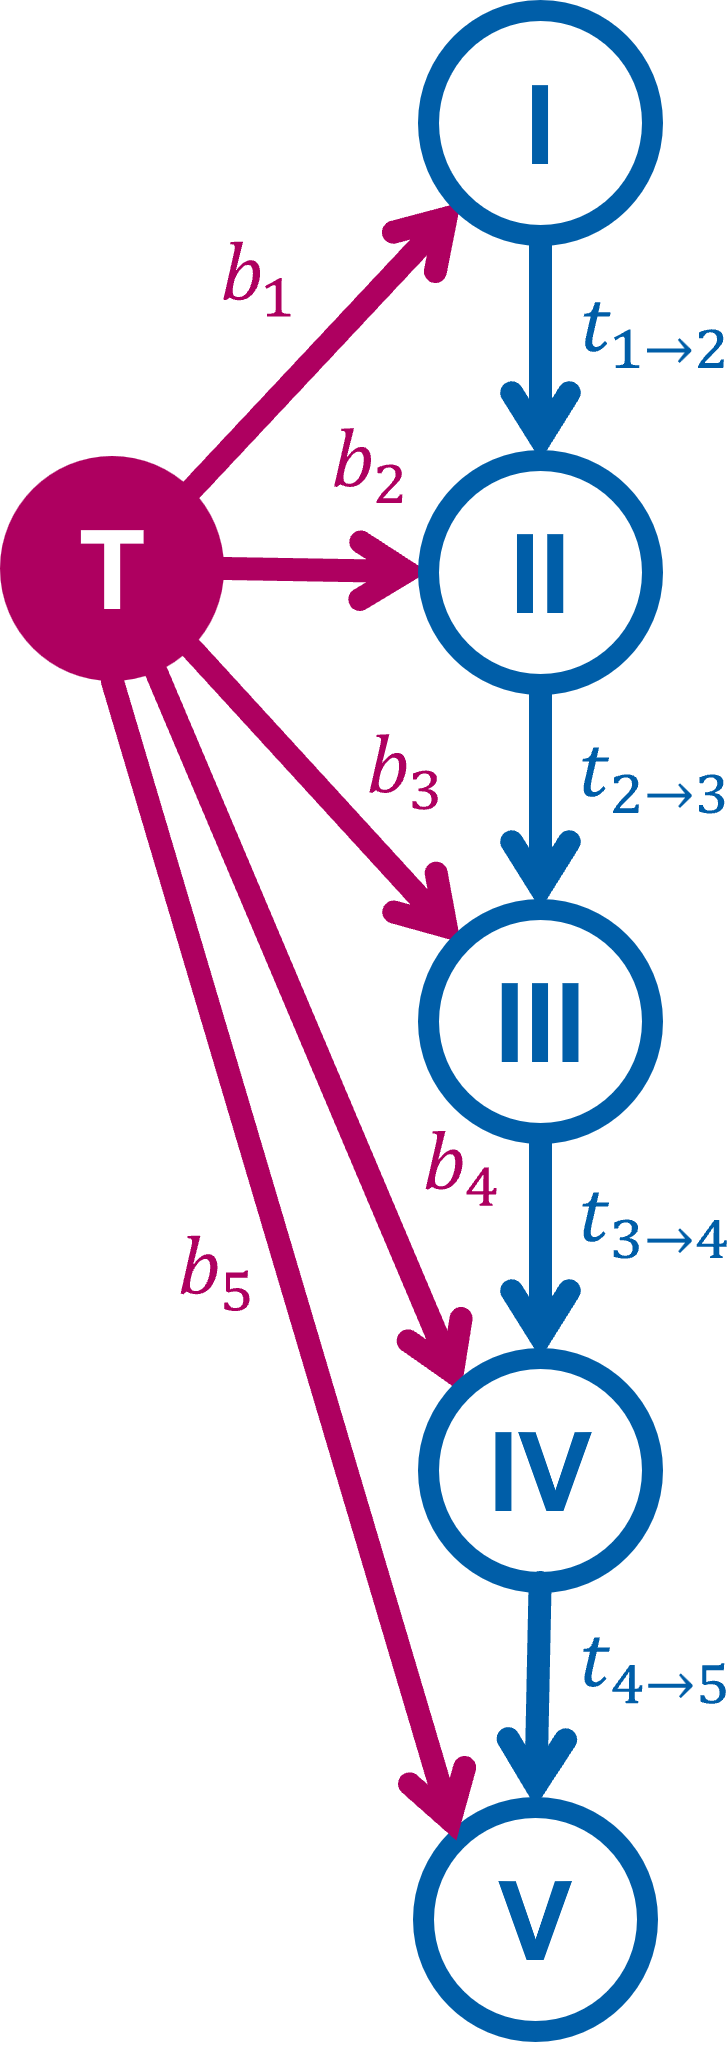
\includegraphics[width=0.2\textwidth,height=\textheight]{figures/Model_5_LNL.png}

}

\caption{\label{fig-graph}Parametrized graphical model of the lymphatic
network considering four LNLs. Blue nodes represent the hidden states of
LNLs \(X_v\), while the red one is the tumor. Arcs represent possible
routes of metastatic spread, associated with a probability.}

\end{figure}%

Now, let \(\boldsymbol{\pi}\) be the \emph{starting distribution}

\begin{equation}\phantomsection\label{eq-starting-distribution}{
\boldsymbol{\pi} = \begin{pmatrix} \pi_i \end{pmatrix} = P \left( \mathbf{X}[0] = \boldsymbol{\xi}_i \right)
}\end{equation}

denoting the probability to start in state \(\boldsymbol{\xi}_i\) at
time step 0. Assuming that every patient started with all LNLs being
healthy, we set \(\pi_i\) to zero for all states except the completly
healthy state
\(\boldsymbol{\xi} = \begin{pmatrix} 0, 0, 0, 0, 0 \end{pmatrix}\),
which has probability one.

Using the quantities introduced so far, the probability
\(P \left( \mathbf{X}[t]=\boldsymbol{\xi}_i \right)\) to be in state
\(\boldsymbol{\xi}_i\) in time step \(t\) can now be conveniently
expressed as a matrix product:

\begin{equation}\phantomsection\label{eq-evolution}{
P \left( \mathbf{X}[t]=\boldsymbol{\xi}_i \right) = \left( \boldsymbol{\pi} \cdot \mathbf{A}^t \right)_i
}\end{equation}

This evolution implicitly marginalizes over all possible paths to arrive
at state \(\boldsymbol{\xi}_i\) after \(t\) time-steps. Additionally, we
must marginalize over the unknown time of diagnosis using a time-prior
\(P_T(t)\) which is defined by a binomial distribution. The t-stage of
the tumor can be included in the model by choosing different
parameterizations of the binomial distribution, considering that a tumor
in late t-stages was diagnosed later than a tumor in early t-stages,
therefore shifting the probability of diagnosis to later time steps.
This finally defines the probability distribution over all states of
lymph node involvement.

\begin{equation}\phantomsection\label{eq-marginalized-evolution}{
P \left( \mathbf{X}=\boldsymbol{\xi}_i \mid \boldsymbol{\theta}, \mathbf{T} \right) = \sum_{t=0}^{t_\text{max}} P_T(t) \left( \boldsymbol{\pi} \cdot \mathbf{A}^t \right)_i
}\end{equation}

where \(\boldsymbol{\theta}=\{ b_v, t_{v \rightarrow v+1} \}\) denotes
the set of all model parameters (7 in our case). Fortunately, the exact
length and shape of this distribution has little impact as previously
shown \citep{ludwig_hidden_2021}. We set \(t_\text{max}=\) 10 and
\(P_\text{early}(t)\) to a binomial distribution with parameter 0.3.
Further details on the HMM can be found in \citet{ludwig_hidden_2021}
and \citet{zora231470}.

With equation~\ref{eq-marginalized-evolution} we can compute the
probability of a patient being in any state \(\xi_i\). Therefore the
likelihood of observing a the For model training we assume that the
diagnoses in our data \(\mathbf{D}\) we observe correspond to the hidden
state \(\mathbf{X}\) of the patient. Thus, learning the model parameters
corresponds to maximizing the probability of observing the dataset
\(\mathbf{D}\):

\begin{equation}\phantomsection\label{eq-likelihood-HMM}{
P \left( \mathbf{D} \mid \boldsymbol{\theta}, \boldsymbol{\pi}\right) = \prod_i \prod_j \left[P \left( \mathbf{X}=\boldsymbol{\xi}_i \mid \boldsymbol{\theta}, T_j \right) \right]^{N_{ij}}
}\end{equation}

In equation~\ref{eq-likelihood-HMM} we take the likelihood of observing
a patient in t-stage \(T_j\) and with involvement \(\xi_i\) to the power
of \(N_{ij}\), corresponding to the number of observations of the
patients in state \(i\) and t-stage \(T_j\) (either early or late) in
the dataset \(\mathbf{D}\).

\section{Mixture Model for Lymphatic Spread}\label{sec-mixture}

Primary tumors at different subsites exhibit distinct lymphatic spread
patterns. This presents a challenge when attempting to generalize
predictive models across subsites. One approach, as introduced in
\citep{ludwig_dynamic_2021}, uses a Hidden Markov Model (HMM) trained
specifically for oropharyngeal cancer. However, extending this model to
other subsites would either require generalizing over several subsites
or training a separate model for each. The former approach sacrifices
precision, particularly for subsites with fewer patients, while the
latter approach becomes computationally intensive and introduces large
uncertainties for subsites with limited patient data, such as C04 (Floor
of mouth) or C05 (Palate).

To address these challenges and exploit the anatomical similarities
between nearby subsites, we introduce a mixture model that combines data
from all subsites into a single model. This model accounts for
anatomical proximities, thereby improving predictive power while
maintaining computational efficiency.

\subsection{Mixture Model Formulation}\label{mixture-model-formulation}

The mixture model assumes that the data is generated by a set of \(M\)
different underlying models. In our case, we introduce \(M\) distinct
lymphatic spread models. Each patient \(k\) is assumed to be generated
by one specific model from this set of \(M\) models.

To formalize this, each patient \(k\) can be assigned to a specific
model via a binary latent vector \(\boldsymbol{\epsilon}_k\). The vector
\(\boldsymbol{\epsilon}_k\) has length \(M\), with exactly one element
set to 1, indicating which model generated the patient's data, and all
other elements set to 0. Thus, for patient \(k\), the latent variable
\(\boldsymbol{\epsilon}_k\) can be interpreted as a categorical
indicator variable that encodes the assignment to one of the \(M\)
lymphatic spread models.

Next, we introduce subsite-specific mixing parameters
\(\boldsymbol{\pi}^s = \{\pi_1^s, \pi_2^s, \dots, \pi_M^s\}\), where
each \(\pi_m^s\) represents the prior probability that a patient with
tumors in subsite \(s\) is generated by model \(m\). These mixing
parameters must satisfy the condition:

\[
\sum_{m=1}^M \pi_m^s = 1, \quad \forall s
\]

The mixing parameters \(\boldsymbol{\pi}^s\) determine the proportion of
patients with tumors in subsite \(s\) that are expected to be generated
by each model. Specifically, \(\pi_m^s\) is the probability that a
randomly chosen patient with a tumor in subsite \(s\) is generated by
model \(m\).

The latent variables \(\boldsymbol{\epsilon}_{k}\), on the other hand,
are patient-specific and represent the assignment of each patient to a
particular model. We will later generalize patients with the same
diagnosis to the latent variable \(\boldsymbol{\epsilon}_{i,j}\). The
subscripts \(i\) and \(j\) represent that the latent variables are only
dependent on the diagnosis of the patient, which consists of lymphatic
involvement \(\boldsymbol{\xi}_i\) and t-stage \(T_j\). The latent
variables are central to the model, as they are hidden (unobserved) and
must be inferred.

The joint probability of the observed data \(\mathbf{D}\) (i.e., patient
data) and the latent variables \(\boldsymbol{\epsilon}\) is given by:

\begin{equation}\phantomsection\label{eq-complete-likelihood}{
P(\mathbf{D}, \boldsymbol{\epsilon} | \boldsymbol{\theta}, \boldsymbol{\pi}) = \prod_{k=1}^{K} \prod_{m=1}^{M} \left[ \pi_m^s P(\mathbf{D}_k | \boldsymbol{\theta}_m, \boldsymbol{\pi}) \right]^{\epsilon_{k}^m}
}\end{equation}

Here:

\begin{itemize}
\tightlist
\item
  \(\pi_m^s\) is the mixing parameter for subsite \(s\) and model \(m\),
\item
  \(P(\mathbf{D}_k | \boldsymbol{\theta}_m)\) is the likelihood of
  patient \(k\)'s data given that it was generated by model \(m\),
\item
  \(\boldsymbol{\theta}_m\) represents the parameters of model \(m\),
\item
  \(\epsilon_{k}^m\) is the latent variable that indicates whether
  patient \(k\) was generated by model \(m\).
\end{itemize}

\textbf{Incomplete data likelihood which can probably be skipped}

Since the latent variables \(\boldsymbol{\epsilon}_k\) are unobserved,
the incomplete complete data likelihood marginalizes over all possible
latent assignments to reflect the uncertainty about which model
generated each patient's data:

\[
P(\mathbf{D} | \boldsymbol{\theta}, \boldsymbol{\pi}) = \sum_{\boldsymbol{\epsilon}} P(\mathbf{D}, \boldsymbol{\epsilon} | \boldsymbol{\theta}, \boldsymbol{\pi})
\]

This allows us to integrate out the latent variables
\(\boldsymbol{\epsilon}\), as their true values are unknown.

\textbf{Continues from here}

The latent variables \(\boldsymbol{\epsilon}_k\) are unknown and must be
inferred from the observed data. The mixture model assumes that each
patient is generated by exactly one of the \(M\) models. However, in our
application, this assumption does not reflect continuous or overlapping
behaviors between subsites. Instead, we infer a probabilistic
distribution over the latent variables, given the observed data and
model parameters. The posterior distribution:

\[
P(\boldsymbol{\epsilon}_k | \mathbf{D}_k, \boldsymbol{\theta}, \boldsymbol{\pi})
\]

describes the probability that patient \(k\) was generated by each of
the \(M\) models, allowing for soft assignments where each patient is
associated with multiple models with certain probabilities, as opposed
to being strictly assigned to just one. Given the probability
distribution for the latent variables \(\boldsymbol{\epsilon}_k\), we
compute the expectation value
\(\mathbb{E}[\boldsymbol{\epsilon}_k] = \boldsymbol{\gamma}(\boldsymbol{\epsilon}_k)\)
for each patient to then apply the complete data likelihood given in
equation~\ref{eq-complete-likelihood}.

We can now apply the mixture model to our dataset \(\mathbf{D}\)
comprising the number of patients \(N_{ijs}\) diagnosed with LNL
involvement state \(\mathbf{X} = \boldsymbol{\xi}_i\), t-stage \(T_j\),
with a primary tumor in subsite \(s\).

The likelihood of the complete dataset is then expressed as:

\begin{equation}\phantomsection\label{eq-complete-likelihood-explicite}{
P \left( \mathbf{D} \mid \boldsymbol{\theta}, \boldsymbol{\pi}\right) = \prod_i \prod_j \prod_s \left[ \prod_{m=1}^M \left[ \pi_m^s P_m \left( \mathbf{X}=\boldsymbol{\xi}_i \mid \boldsymbol{\theta}_m, T_j \right) \right]^{\gamma(\epsilon_{i,j}^m)} \right]^{N_{ijs}}
}\end{equation}

In equation~\ref{eq-complete-likelihood} we compute the likelihood of
observing state \(\boldsymbol{\xi}_i\) with t-stage \(T_j\) under model
\(m\) similarly to equation~\ref{eq-likelihood-HMM}. However, we weight
each model with the mixing parameter \(\pi_m^s\). Since the mixing
parameters are subsite dependent, we differ between each subsite.

The model now contains two sets of parameters: the tumor spread
probabilities \(\mathbf{\theta_m}\) for each model, and the mixing
coefficients \(\pi_m^s\). The posterior distribution over these
parameters \(P(\boldsymbol{\theta},\boldsymbol{\pi}|\mathbf{D})\) can be
estimated assuming a uniform prior on the interval {[}0,1{]} for all
parameters. However,
\(P(\boldsymbol{\theta},\boldsymbol{\pi}|\mathbf{D})\) is a
multimodal-distribution as one can permute the different models and
achieve the same result. To address this problem, we apply an
expectation-maximization (EM) algorithm.

\subsection{Expectation-Maximization (EM)
Algorithm}\label{expectation-maximization-em-algorithm}

To solve for the model parameters, we apply the EM algorithm, which
iterates between two steps: the \textbf{Expectation (E) step} and
\textbf{the Maximization (M) step}.

\paragraph{Expectation Step}\label{expectation-step}

In the E-step, we compute the expected value of the latent variables
\(\boldsymbol{\epsilon}\), which represent the probabilities of a
patient \(k\) originating from one of the models \(m\). Given the
current estimates of \(\boldsymbol{\theta}\) and \(\boldsymbol{\pi}\),
the expectation value \(\gamma(\epsilon_m^k)\) is calculated as:

\begin{equation}\phantomsection\label{eq-expectation-step}{
\mathbb{E}[\epsilon^m] = \gamma(\epsilon^m_{i,j}) = \frac{\pi_m^s P(\mathbf{X} = \boldsymbol{\xi}_i \mid \boldsymbol{\theta_m}, T_j)}{\sum_{n=1}^M \pi_n^s P(\mathbf{X} = \boldsymbol{\xi}_i \mid \boldsymbol{\theta_n}, T_j)}
}\end{equation}

THE OTHER OPTION

\begin{equation}\phantomsection\label{eq-expectation-step2}{
\mathbb{E}[\epsilon^m] = \gamma(\epsilon^m_k) = \frac{\pi_m^s P(\mathbf{X} = \boldsymbol{\xi}_k \mid \boldsymbol{\theta_m}, T_k)}{\sum_{j=1}^M \pi_j^s P(\mathbf{X} = \boldsymbol{\xi}_k \mid \boldsymbol{\theta_j}, T_k)}
}\end{equation}

Here, the mixing parameter \(\pi_m^s\) depends on the subsite location
of the primary tumor of patient \(k\).

\paragraph{Maximization Step}\label{maximization-step}

In the M-step, the model parameters are updated by maximizing the
complete data likelihood in equation
equation~\ref{eq-complete-likelihood-explicite}. For better handling, we
are optimizing the log likelihood:

\begin{equation}\phantomsection\label{eq-maximization-step}{
\ln P(\mathbf{D}, \boldsymbol{\epsilon} \mid \boldsymbol{\theta}, \boldsymbol{\pi}) = \sum_{i} \sum_j \sum_{s} N_{i,j,s} \sum_{m=1}^M \gamma(\epsilon^m_{i,j}) \left( \ln \pi_m^s + \ln P(\mathbf{X} = \boldsymbol{\xi}_i \mid \boldsymbol{\theta_m}, T_j) \right)
}\end{equation}

In this step, the mixture parameters \(\pi_m^s\) and the model
parameters \(\boldsymbol{\theta}_m\) can be optimized separately. The
mixture parameters \(\pi_m^s\) can be updated analytically:

\begin{equation}\phantomsection\label{eq-mixture-maximization}{
\pi_m^s = \frac{1}{N^s} \sum_k^{N^s} \gamma(\epsilon^m_k)
}\end{equation}

On the other hand, the model parameters \(\boldsymbol{\theta_m}\) are
optimized component-wise using an optimization algorithm, as an analytic
solution is not feasible. The updated log-likelihood for each model is:

\[
\ln P(\mathbf{D}, \boldsymbol{\epsilon} \mid \boldsymbol{\theta}_m) = \sum_{i} \sum_j \gamma(\epsilon^m_{i,j}) \ln P(\mathbf{X} = \boldsymbol{\xi}_i \mid \theta_m, T_j)
\]

By iterating these steps, the EM algorithm converges to a (local)
maximum of the complete data likelihood
equation~\ref{eq-complete-likelihood}.

\section{Three component Mixture Model}\label{sec-3comp}

We illustrate the methodology for a mixture model with M = 3 components,
considering the ipsilateral involvement of LNLs I, II, III, IV, and V.
We include the ICD codes as subsites for oral cavity, hypopharynx and
oropharynx. In figure~\ref{fig-convergence} the convergence of the
negative log-likelihood and change in model parameters is depicted.
After a random inizialization, the algorithm rapidly converges. The
algorithm was stopped when the difference of log-likelihood between two
iterations was below 0.01.

\begin{figure}

\centering{

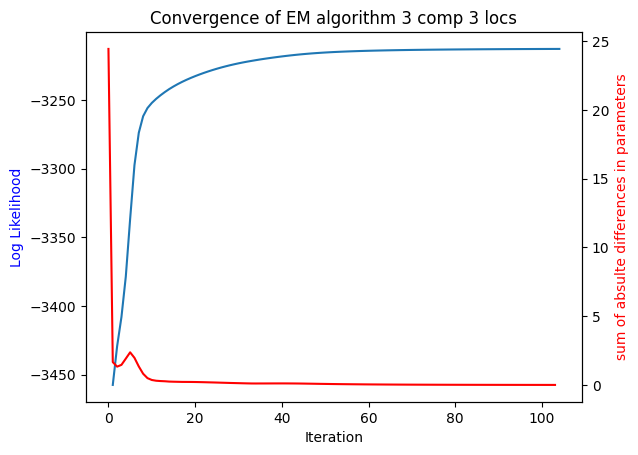
\includegraphics{figures/Convergence_3_comp.png}

}

\caption{\label{fig-convergence}The y-axis on the left shows the
negative likelihood convergence depicted in the blue line. The y-axis on
the right shows the sum of absulte difference between all model
parameters showing that the parameter values stabilize rapidly as well.}

\end{figure}%

In figure~\ref{fig-3_simplex}, we visualize the resulting mixture
coefficients \(\boldsymbol{\pi}\) using a spatial representation, where
the vertices of the triangle correspond to the three components. In
figure~\ref{fig-3-matrix}, these mixture coefficients are presented in
matrix form, with the y-axis representing the ICD codes, showing how the
mixture components in each row add up to 1.

The spatial plot in figure~\ref{fig-3_simplex} illustrates how the model
assigns the three components to different tumor subsites. Component 0,
located at the bottom right of the triangle, primarily characterizes
oropharyngeal subsites. For instance, the base of tongue subsite (C01),
which exhibits the highest involvement of LNL II, is fully assigned to
this component. Similarly, subsite C10, which includes several
oropharyngeal regions, is assigned roughly 50\% to the oropharynx-like
component, with the remaining mixture distributed across the other two
components.

Hypopharyngeal subsites, on the other hand, are fully assigned to
Component 2, located at the top vertex of the triangle. Meanwhile, the
gum subsite (C03), with predominant LNL I involvement, is entirely
assigned to Component 1, situated at the bottom left. As subsites
anatomically approach the oropharynx, their mixture coefficients for the
oropharynx-like component increase. This is evident in the subsites C02
(tongue) and C05 (palate), which display a higher proportion of
oropharyngeal influence in their mixture. These results conform well
with the involvement patterns observed in the data.

\begin{figure}

\begin{minipage}{0.71\linewidth}

\begin{figure}[H]

\centering{

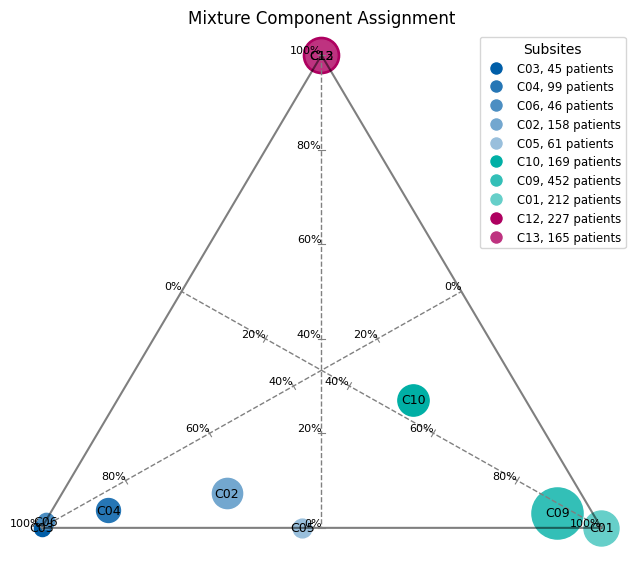
\includegraphics{figures/mixture_components_3_simplex_t_stages_new.png}

}

\caption{\label{fig-3_simplex}Assignment of each subsite to each of the
three components. The closer a subsite is to a vertex, the more it is
assigned to the corresponding component, with component 0 on the bottom
right, 1 on the bottom left and 2 on the top. The size of the marker
(area) corresponds to the number of patients in each subsite.}

\end{figure}%

\end{minipage}%
%
\begin{minipage}{0.29\linewidth}

\begin{figure}[H]

\centering{

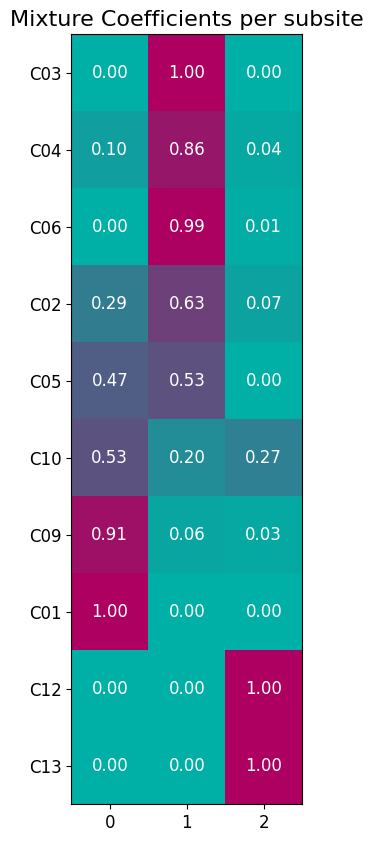
\includegraphics{figures/mixture_components_3_t_stages_new.png}

}

\caption{\label{fig-3-matrix}Matrix representation of component
assignment. Each row of the matrix corresponds to each ICD code. The
collums represent the three different components}

\end{figure}%

\end{minipage}%

\end{figure}%

\section{Four component Mixture Model}\label{sec-4comp}

We can extend the mixture model to include the larynx. The larynx
patients are more finely divided into ICD codes C32.0, C32.1 and C32.2
as there is a notable difference between these ICD codes in
figure~\ref{fig-involvement}.

Simlarly to the three component model, we can analyze the convergence
over the iterations of the EM-algorithm. In
figure~\ref{fig-convergence4} we can see that in this more complex
model, the likelihood space becomes more complex as at around 200
iterations, the negative log-likelihood starts to increase faster again.

\begin{figure}

\centering{

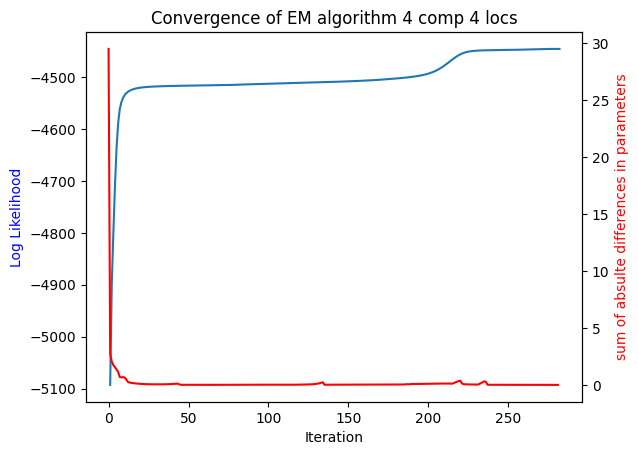
\includegraphics{figures/convergence_4_components_4_loc.png}

}

\caption{\label{fig-convergence4}The y-axis on the left shows the
negative likelihood convergence depicted in the blue line. The y-axis on
the right shows the sum of absulte difference between all model
parameters.}

\end{figure}%

The component assignment is shown in figure~\ref{fig-4-matrix}.
Similarly to the 3-component model the different tumor locations are
assigned to a one of the components\ldots.

Here i probably should permute the components such that we have the same
ordering as in the 3-component model.

\begin{figure}

\centering{

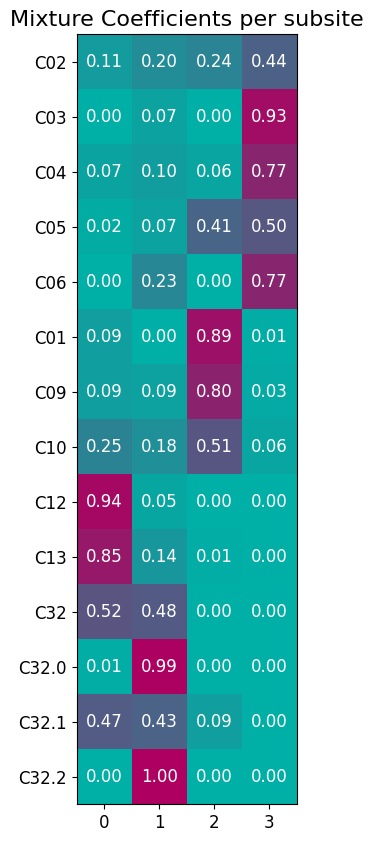
\includegraphics{figures/mixture_components_4_t_staging_add_larynx.png}

}

\caption{\label{fig-4-matrix}Matrix representation of component
assignment. Each row of the matrix corresponds to each ICD code. The
collums represent the three different components}

\end{figure}%

--\textgreater{} Add predictions and compare to the prevalence.
Additionally we could compare to tumor location predictions.


  \bibliography{references.bib}



\end{document}
